\documentclass[tikz,border=10pt]{standalone}
\usepackage{tikz}
\usetikzlibrary{positioning}
\usepackage{tikz-feynman}
\begin{document}

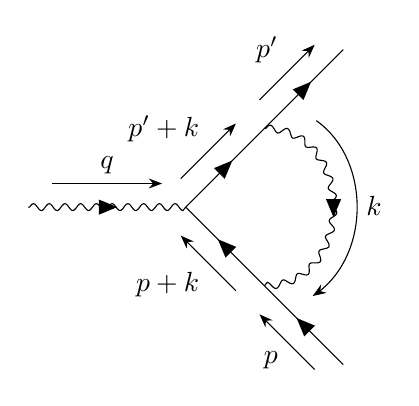
\begin{tikzpicture}[scale=0.5]
	\begin{feynman}
		%% fig a
		\vertex (a1) at (0,0);
		\vertex[above right = 0 and 2 of a1] (a2);
		\vertex[above right = 2 and 4 of a1] (a3);
			\vertex[above right = -2 and 4 of a1] (a4);
		\vertex[above right = 1 and 3 of a1] (a3m);
		\vertex[above right = -1 and 3 of a1] (a4m);
		% 对各个顶点连线
		\diagram*{
		(a4) --[fermion,momentum=\(p\)] (a4m)--[fermion,momentum=\(p+k\)] (a2)
		--[fermion,momentum=\(p^{\prime}+k\)] (a3m)--[fermion,momentum=\(p^{\prime}\)] (a3);
		(a1)--[charged boson,momentum=\(q\)](a2);
		(a3m) -- [charged boson,out=90,in=90,looseness=1.5,relative,momentum=\(k\)](a4m);
		};
	\end{feynman}
\end{tikzpicture}

\end{document}